\documentclass{standalone}
\usepackage{tikz}

\begin{document}
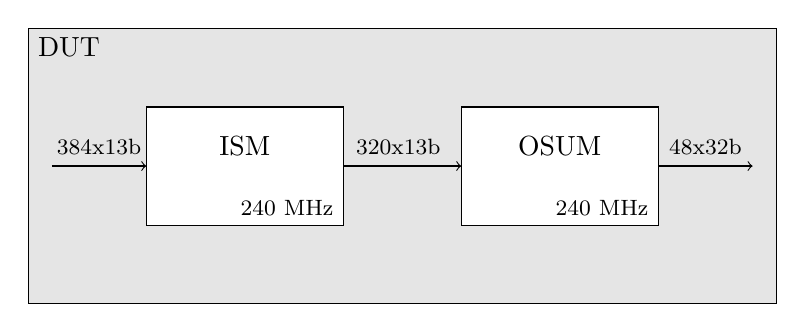
\begin{tikzpicture}

    % Background rectangle with borders (larger)
    \draw[fill=gray!20] (-1.5,-1) rectangle (8,2.5);

    % "DUT" at the top left of the background rectangle
    \node[anchor=north west] at (-1.5,2.5) {DUT};

    % ISM rectangle (larger)
    \draw[fill=white] (0,0) rectangle (2.5,1.5);
    \node at (1.25,1) {ISM};
    \node[anchor=south east] at (2.5,0) {\footnotesize 240 MHz};

    % OSUM rectangle (larger and shifted right)
    \draw[fill=white] (4,0) rectangle (6.5,1.5);
    \node at (5.25,1) {OSUM};
    \node[anchor=south east] at (6.5,0) {\footnotesize 240 MHz};

    % Arrow from ISM to OSUM (adjusted to touch borders)
    \draw[->] (2.5,0.75) -- (4,0.75);
    \node at (3.2,1) {\footnotesize 320x13b};

    % Arrow going into ISM
    \draw[->] (-1.2,0.75) -- (0,0.75);
    \node at (-0.6,1) {\footnotesize 384x13b};

    % Arrow going out of OSUM
    \draw[->] (6.5,0.75) -- (7.7,0.75);
    \node at (7.1,1) {\footnotesize 48x32b};

\end{tikzpicture}
\end{document}